%!TEX root = avollmer.tex

\section{The Co-Construction Game}
% \section{Method}

With the aim that improving our understanding of how humans negotiate protocols of interaction could provide hints on how robots could do it also, we designed a new experimental setup which allows constraining the communication channels between two partners in asymmetric roles who should collaborate in order to achieve a joint construction task. 
%We consider a joint construction where only one participant is aware of the targeted construction (the architect) while only the other has the ability to achieve it (the builder). The communication between partners is reduced to the use of symbolic events that the architect can send to the builder. 
% the builder can sed all kinds of non-verbal signals to the architect. only one way of communication is really restricted
%Neither the architect nor the builder are given any a priori information on the meaning of the symbolic signals and should agree on the meaning of such signals by the mean of the construction task.
This section describes the details of the experimental setup, the participants we recruited for the current pilot study, and the protocol used for running the study.

\subsection{Setup}

\begin{figure}[!ht]
\centering
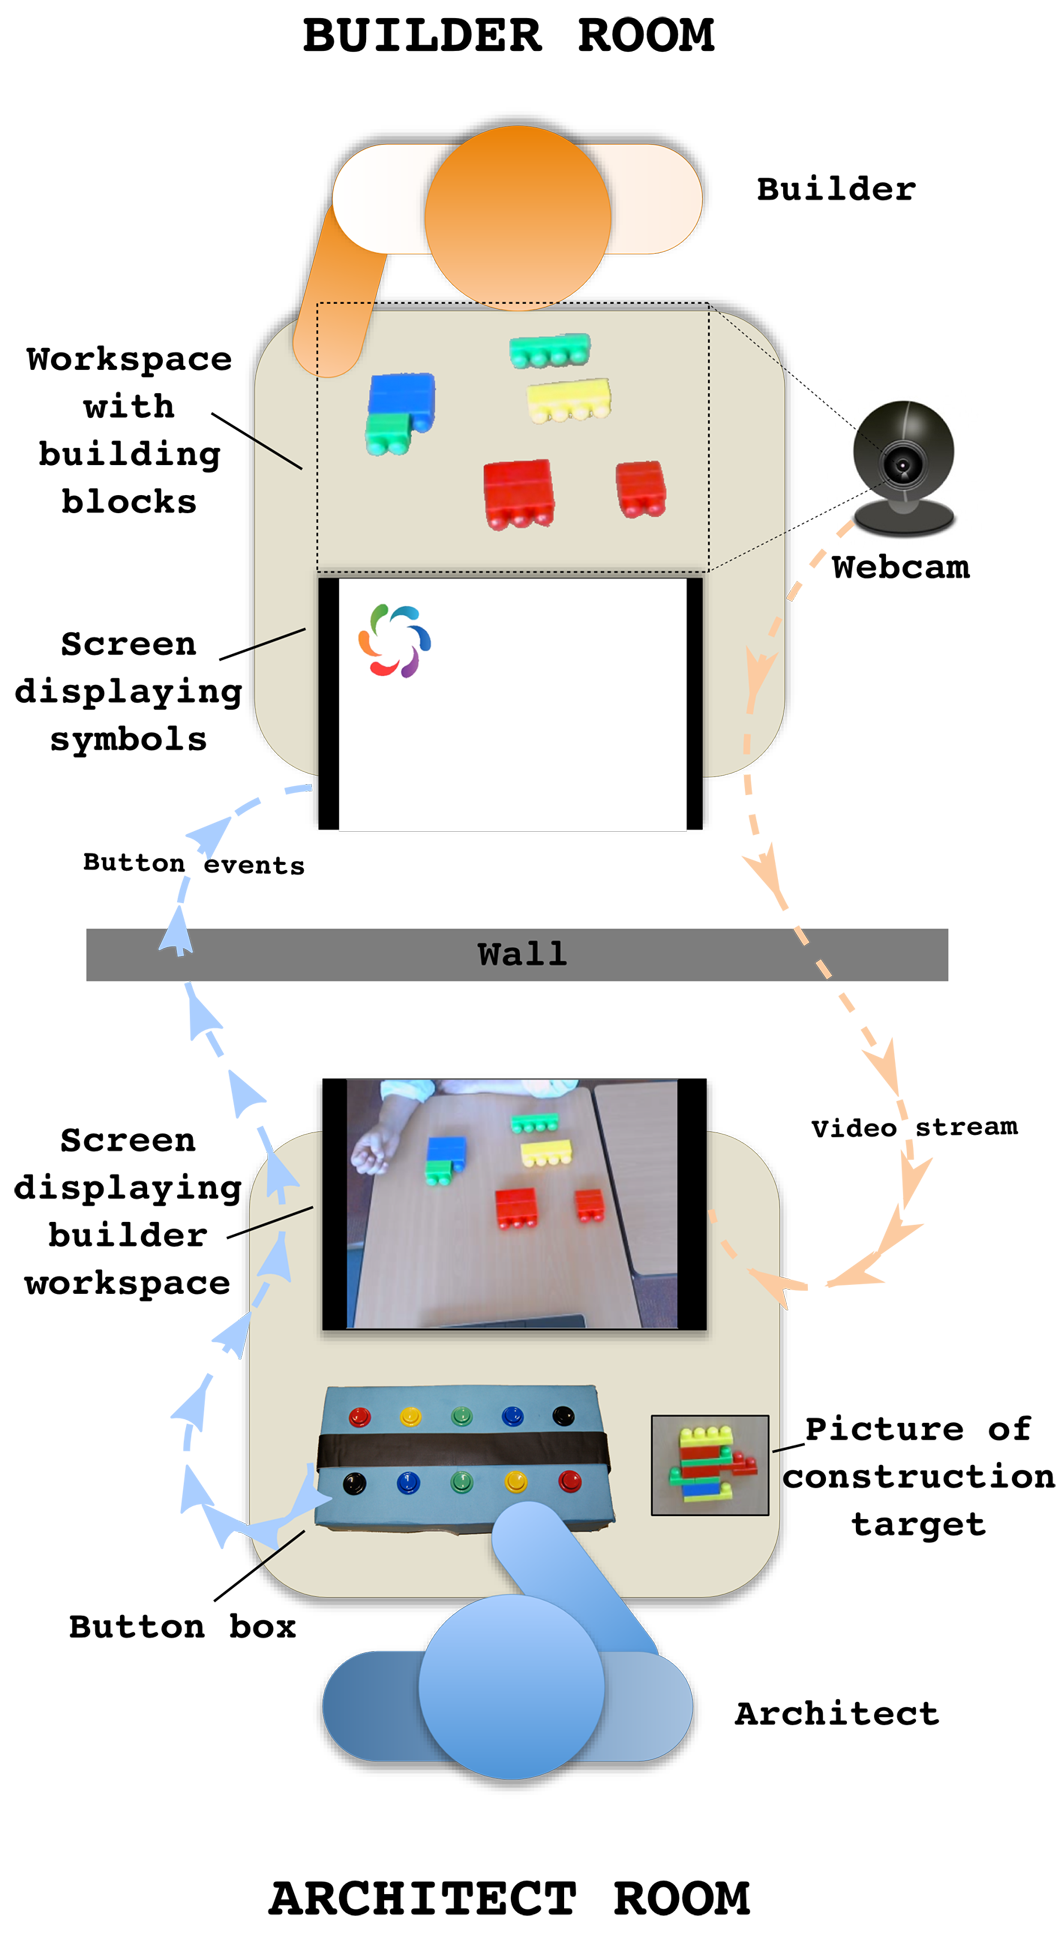
\includegraphics[width=0.8\columnwidth]{media/plots/setup_normal_video_one_columnscaled}%
\caption{Schematic view of our experimental setup. An architect (bottom) and a builder (top) should collaborate in order to build the construction target while located in different rooms. The architect has a picture of the targeted construction, while the builder has access to the construction blocks. The communication between them is restricted. The architect only sees a top view of the builder's workspace and can communicate with the builder only though the use of 10 buttons which, when pressed, display symbols on a screen on the builder side.}
\label{fig:overviewsetup}
\end{figure}

Figure~\ref{fig:overviewsetup} gives an overview of the experimental setup which considers an architect and a builder that are each seated at a table in front of a computer screen in two separate rooms and can neither hear nor see each other. 

The builder is equipped with a set of building blocks, in our case with 12 primary-colored Mega Bloks\textsuperscript{\textregistered} toy blocks differing in shape and color (see Figure~\ref{fig:bricks}). %\todo{maybe we can remove the following they are all on the figure: There were three red two-pads, two red three-pads, two yellow four-pads, two blue three-pads, two green two-pads, and one green four-pads blocks.} 
The goal of the game is to assemble a specific construction yet unknown to the builder. As exemplified in Figure~\ref{fig:structures}, a construction is a flat combination of several blocks at least linked to one another by one pad. It does not necessarily contain all available blocks.

\begin{figure}[!ht]
\centering
\subfigure[][The box and the buttons used as an interface for the architect to communicate with the builder.]{\label{fig:box}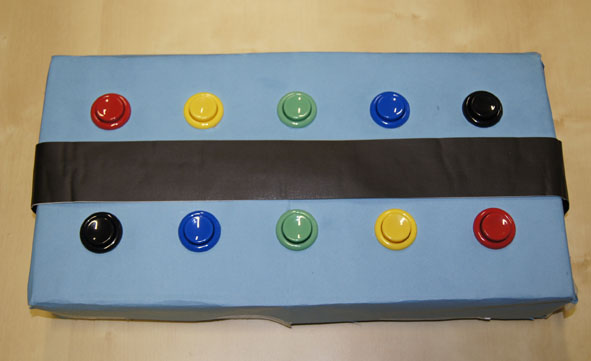
\includegraphics[width=0.45\columnwidth]{media/boxscaled}}\qquad
\subfigure[][All toy blocks used in the collaborative construction task.]{\label{fig:bricks}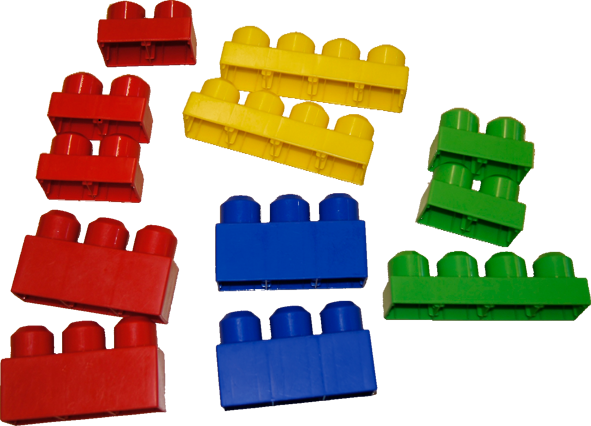
\includegraphics[width=0.45\columnwidth]{media/bricksscaled}}\\
\subfigure[][Three examples of the 20 target structures presented to the architect.]{
    \label{fig:structures}
    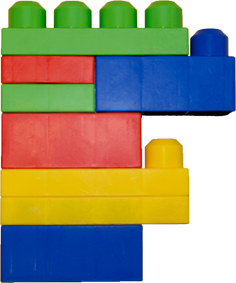
\includegraphics[height=0.2\columnwidth]{media/structures/1scaled}
    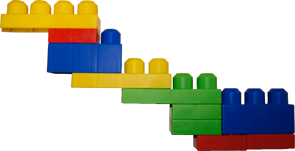
\includegraphics[height=0.2\columnwidth]{media/structures/2scaled}
    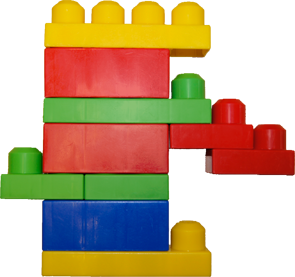
\includegraphics[height=0.2\columnwidth]{media/structures/3scaled} 
}
\caption{}
\end{figure}

% \begin{figure}[!ht]
%     \centering
%     \subfigure[][]{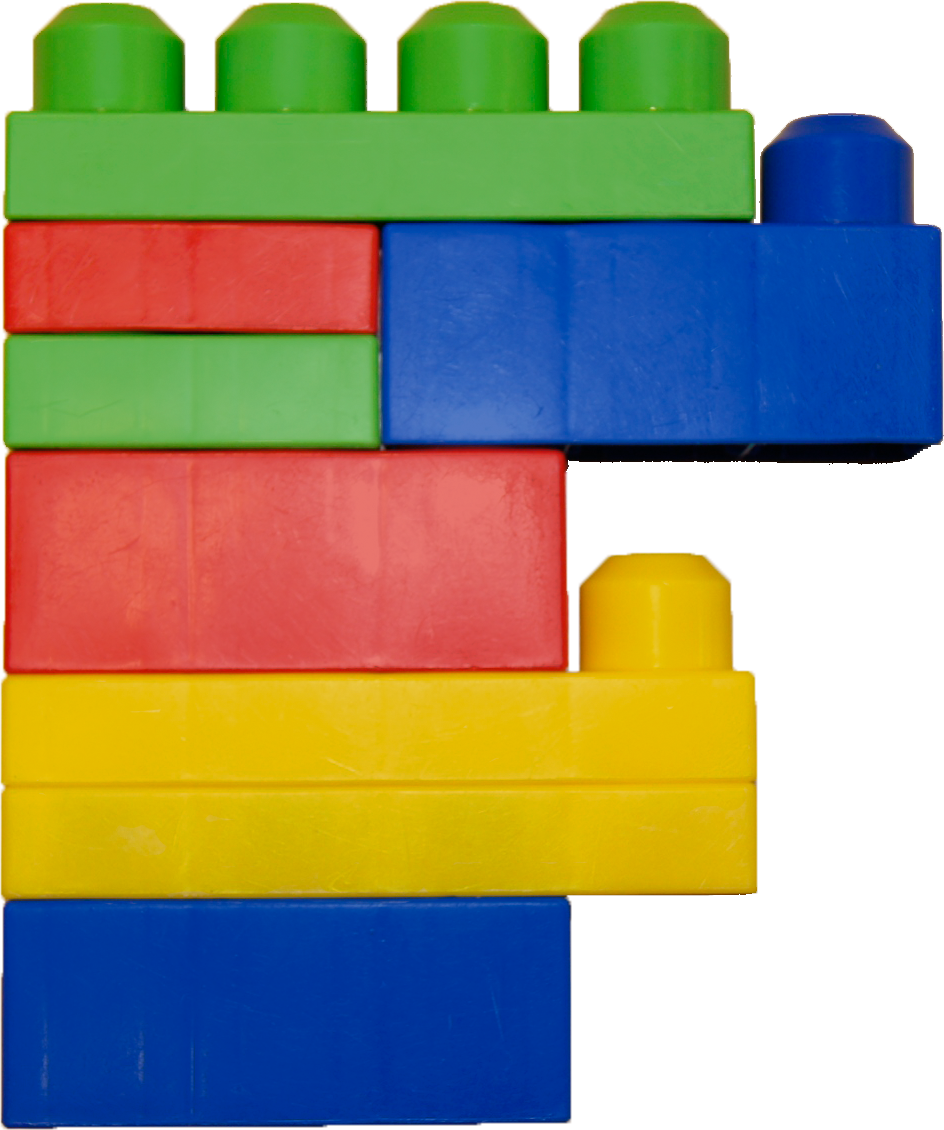
\includegraphics[height=0.2\columnwidth]{media/structures/1}}\
%     \subfigure[][]{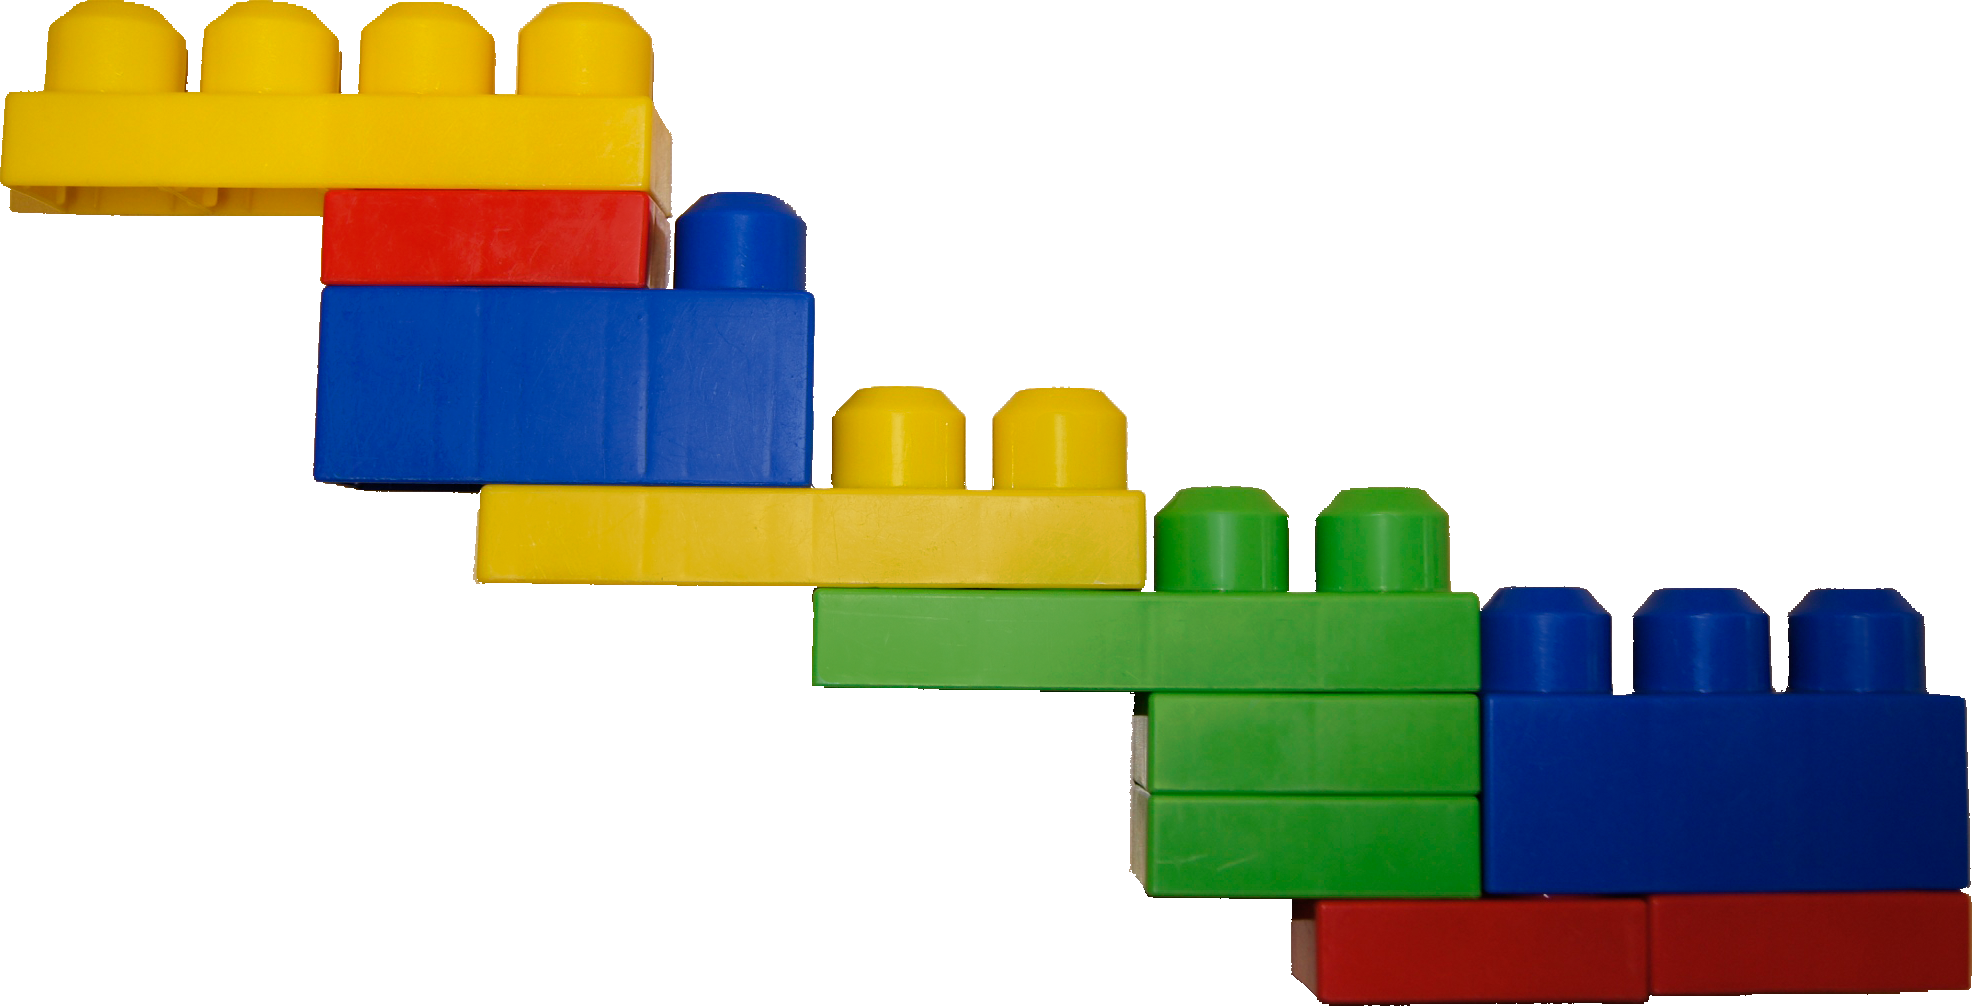
\includegraphics[height=0.2\columnwidth]{media/structures/2}}\
%     \subfigure[][]{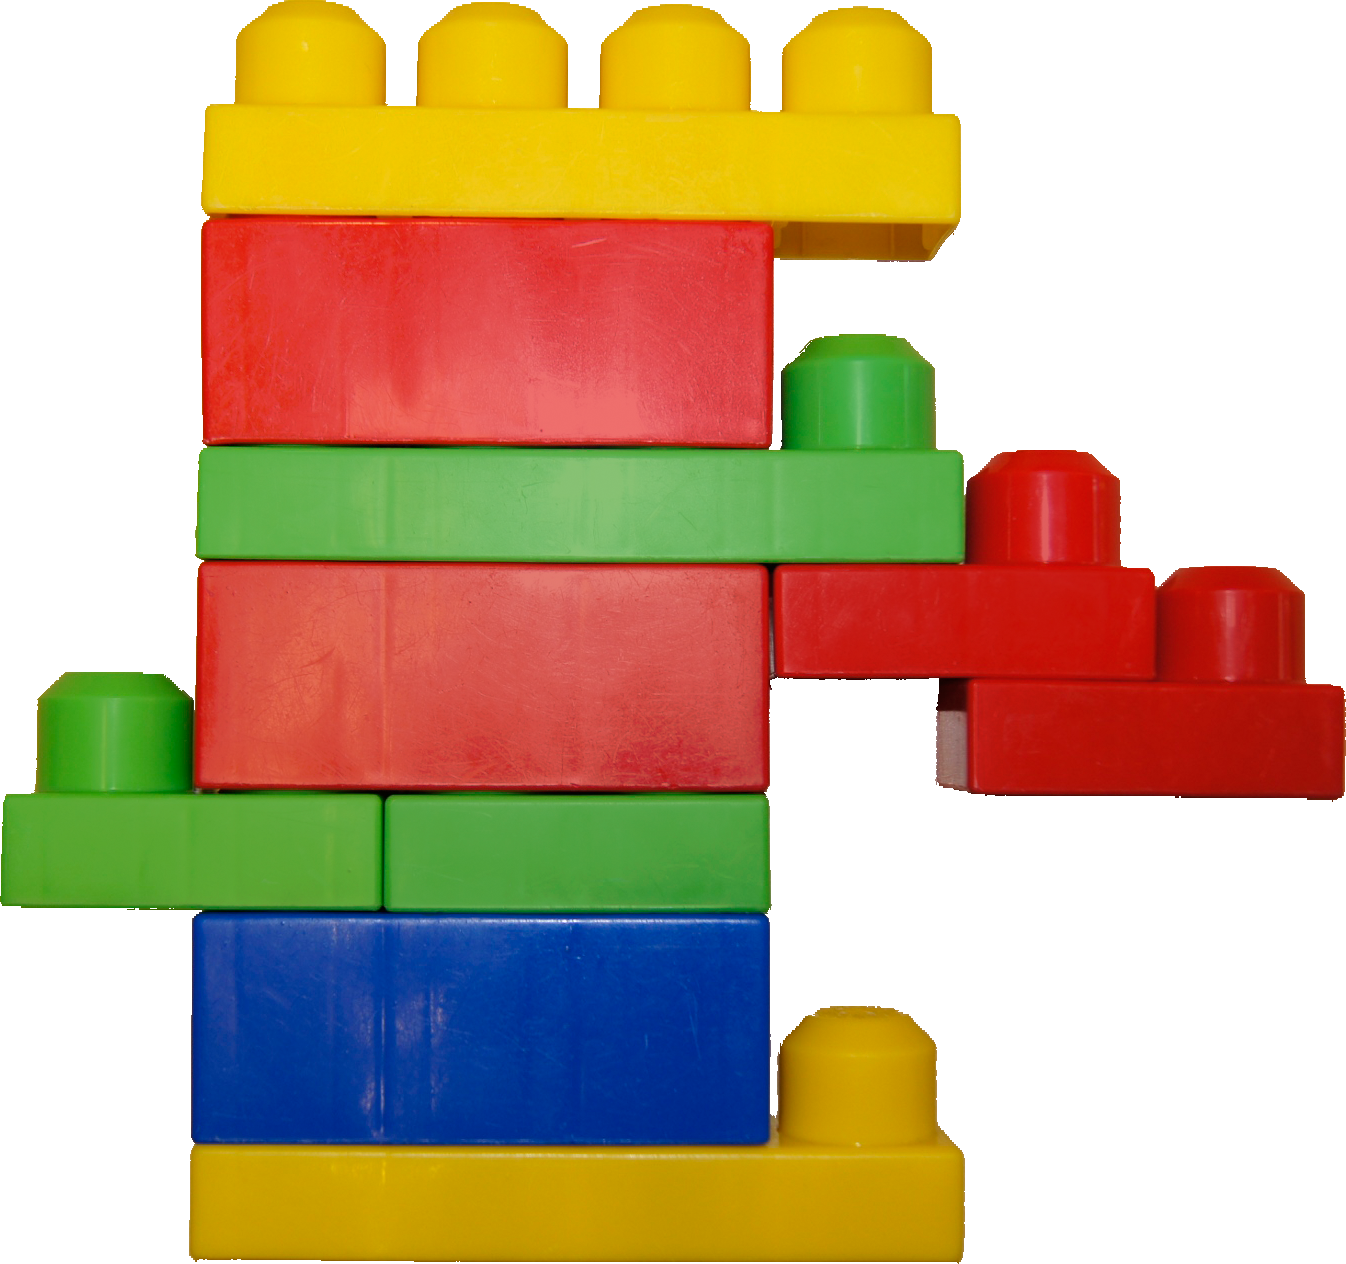
\includegraphics[height=0.2\columnwidth]{media/structures/3} \label{fig:sc}}%
%     \caption{Three examples of target structures presented to the architect.} 
%     \label{fig:structures}
% \end{figure}

The architect is given an image of the specific construction to be build and is told to guide the other player building it. A screen displays a live top view of the builder workspace. To communicate with the builder, the architect has access to a rudimentary interface made of 10 buttons, see Figure~\ref{fig:box}. Pressing a button displays a symbol on the screen located in the builder room. Each button is mapped to one of ten symbols and one of ten positions (two rows of five symbols) on the builder's screen, whereby the spacial organization of buttons differs from the spatial organization of displayed symbols. The mapping is randomized for each subject and fixed for the duration of one game. Figure~\ref{fig:sign} shows the different symbols.

\begin{figure}[!ht]
\centering

\includegraphics[width=0.8\columnwidth]{media/sign}%
\caption{The ten signs displayed on the builder screen.}
\label{fig:sign}
\end{figure}

\subsection{Participants}

We recruited 22 participants (19 m, 3 f) among students and staff at INRIA Bordeaux Sud-Ouest. Their age range was between 20 and 35 ($M = 25, SD = 3.91$) years. They played the collaborative game in pairs, where the two players in a pair were assigned randomly to the roles of a builder and an architect. Seven of the eleven pairs played the game together twice, such that each of the 14 participants involved assumed each role once. One second round of a dyad was excluded from the analyses, because the architect neglected the task instructions and altered the target structure during the game. This resulted in a total of 17 rounds.

\subsection{Procedure}
\label{sec:procedure}
Participants were not given the chance to talk about the game before it began. Architect and builder were instructed about their respective roles separately in their respective rooms. We presented the architects with a set of 20 pictures of different constructions from which they chose one. The builder was informed about the constraint that applied on the construction, i.e. flat construction which does not necessarily contain all available blocks. Architect and builder were specifically told that the button positions did not directly map onto the symbols' positions displayed on the builder's screen, but that the mapping was fixed and arbitrary. Additionally, because the architect could see the hands of the builder during the game (see Figure~\ref{fig:overviewsetup}), the builder is told to only use his/her hands to move blocks and not to use hand signs. In practice, this was well respected by participants.

The game was \textbf{not} preceded by any training sessions. We aimed at reducing the time between the instruction of the participants and the beginning of the game as much as possible, so that they did not have time to elaborate any concrete strategy before the game began. 

Once the game started, we observed the behavior of the two players and asked them to speak aloud about the meaning associated to the symbols/buttons. The experimenters took notes on the participants' remarks. The experiment stopped only when the builder decided and told the experimenters that the structure he had build was correct.

%During the experiments, the architects and builders were ask to speak aloud respectively what meaning they intended to convey by pressing a button and what they understood from the symbols displayed on the screen. 

